\documentclass[11pt,aspectratio=169]{beamer}

\usetheme{Madrid}
\usecolortheme{default}
\setbeamertemplate{navigation symbols}{}
\setbeamertemplate{footline}[frame number]

\usepackage[utf8]{inputenc}
\usepackage[T1]{fontenc}
\usepackage{graphicx}
\usepackage{booktabs}
\usepackage{amsmath}
\usepackage{subcaption}
\usepackage{xcolor}

\newcommand{\PC}{\emph{Plan Cuadrante}}

\title[Beat Policing and Police Effectiveness]{Boots in the Beat}
\subtitle{Effects of Beat Policing on Victimization and Crime Perception}
\author[Garc\'ia-Hombrados]{Andr\'es Barrios-Fern\'andez \and Jorge Garc\'ia-Hombrados \and Daniel P\'erez-Parra \\[4pt] \small{Presented by Jorge Garc\'ia-Hombrados}}
\institute[UAM]{Universidad Aut\'onoma de Madrid}
\date{Universidad Carlos III de Madrid \\ September 23, 2026}

\begin{document}

% -----------------------------------------------------------------
\begin{frame}
\titlepage
\end{frame}

\begin{frame}{Outline}
\tableofcontents
\end{frame}

% ===================================================================
\section{Motivation}
% ===================================================================

\begin{frame}{Motivation}
\begin{itemize}
\item Crime is a top public concern and a major driver of public and private spending worldwide.
\item We know a lot about \textbf{how many} police resources reduce crime.
\item We know much less about \textbf{how those resources are deployed}.
\begin{itemize}
\item Same number of officers, organized differently across space, may perform very differently.
\end{itemize}
\item \textbf{Beat policing}: permanently assigning officers to small, fixed territorial units, rather than rotating them across a larger area.
\begin{itemize}
\item Widely adopted around the world.
\item Rigorous causal evidence on its effects remains scarce.
\end{itemize}
\end{itemize}
\end{frame}

\begin{frame}{This Paper}
\begin{itemize}
\item We study \textbf{\PC}, a large-scale beat-policing reform in Chile.
\item It subdivided municipalities into smaller \textbf{quadrants} and permanently assigned officers to them.
\item We exploit the \textbf{staggered rollout} of the program (1998--2013) across Chilean municipalities.
\item Rich administrative \textbf{and} household survey data let us look at:
\begin{itemize}
\item Actual crime (victimization, reported crime, arrests)
\item Perceived security (crime perception, trust, private security investment)
\end{itemize}
\item We separate the \textbf{deployment/strategy} channel from the \textbf{resources} channel.
\end{itemize}
\end{frame}

\begin{frame}{Preview of Results}
\begin{columns}[T]
\column{0.5\textwidth}
\textbf{Crime and safety}
\begin{itemize}
\item Victimization: $-$10 pp (36\%)
\item Reported crime: $-$10\% (208 per 100k)
\item Arrests: $+$14\% (48 per 100k)
\end{itemize}
\column{0.5\textwidth}
\textbf{Perceptions and behavior}
\begin{itemize}
\item Crime perception: $-$15 pp (36\%)
\item Private security investment: $-$8 pp (37\%)
\item Trust in the police: $\uparrow$
\end{itemize}
\end{columns}
\vspace{8pt}
\begin{itemize}
\item Effects hold in municipalities with \textbf{no differential resource increase}.
\item No evidence of spatial spillovers to neighboring municipalities.
\end{itemize}
\end{frame}

\begin{frame}{Contribution to the Literature}
\begin{enumerate}
\item First causal evidence on \textbf{beat policing} at scale, on both crime \emph{and} security perceptions.
\item Complements the police-organization literature (response times, prioritization, technology) by studying \textbf{territorial deployment} as a distinct margin.
\item Complements the police-resources literature: \textbf{how} resources are organized matters, not only \textbf{how much} there is.
\end{enumerate}
\end{frame}

% ===================================================================
\section{Institutional Setting}
% ===================================================================

\begin{frame}{Carabineros de Chile}
\begin{itemize}
\item National, hierarchical police force; centrally defined doctrine, limited local discretion.
\item Basic operational unit: the \emph{comisar\'ia} --- historically covered the \textbf{entire municipal territory}.
\item Average \emph{comisar\'ia}: 1,608 km$^2$, 57,642 inhabitants.
\end{itemize}
\end{frame}

\begin{frame}{\PC (Plan Cuadrante de Seguridad P\'ublica)}
\begin{itemize}
\item Rolled out 1998--2013 in municipalities with $\geq$70\% urban population (150 eligible municipalities).
\item Subdivided each \emph{comisar\'ia} into $\sim$7 \textbf{quadrants} on average.
\item Officers \textbf{permanently} assigned to one quadrant (vs.\ rotating across the whole municipality).
\item Average quadrant: 185 km$^2$, 13,466 inhabitants, $\sim$3 officers per shift.
\item National operational guidelines unchanged $\Rightarrow$ strategy adjustments emerge \emph{endogenously} from the new deployment, not from a top-down redesign.
\end{itemize}
\end{frame}

\begin{frame}{Rollout of \PC}
\centering
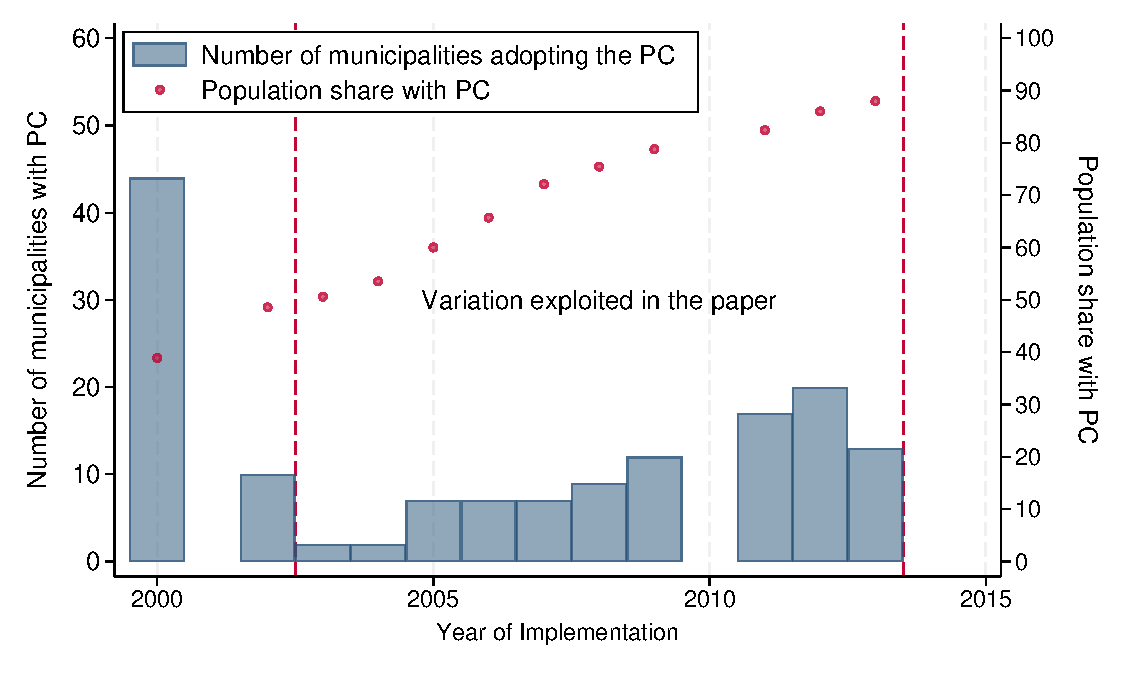
\includegraphics[width=0.85\linewidth]{figures/Graph_PCvariation.pdf}
\end{frame}

\begin{frame}{Illustration: Quadrants in the Concepci\'on Metropolitan Area}
\centering
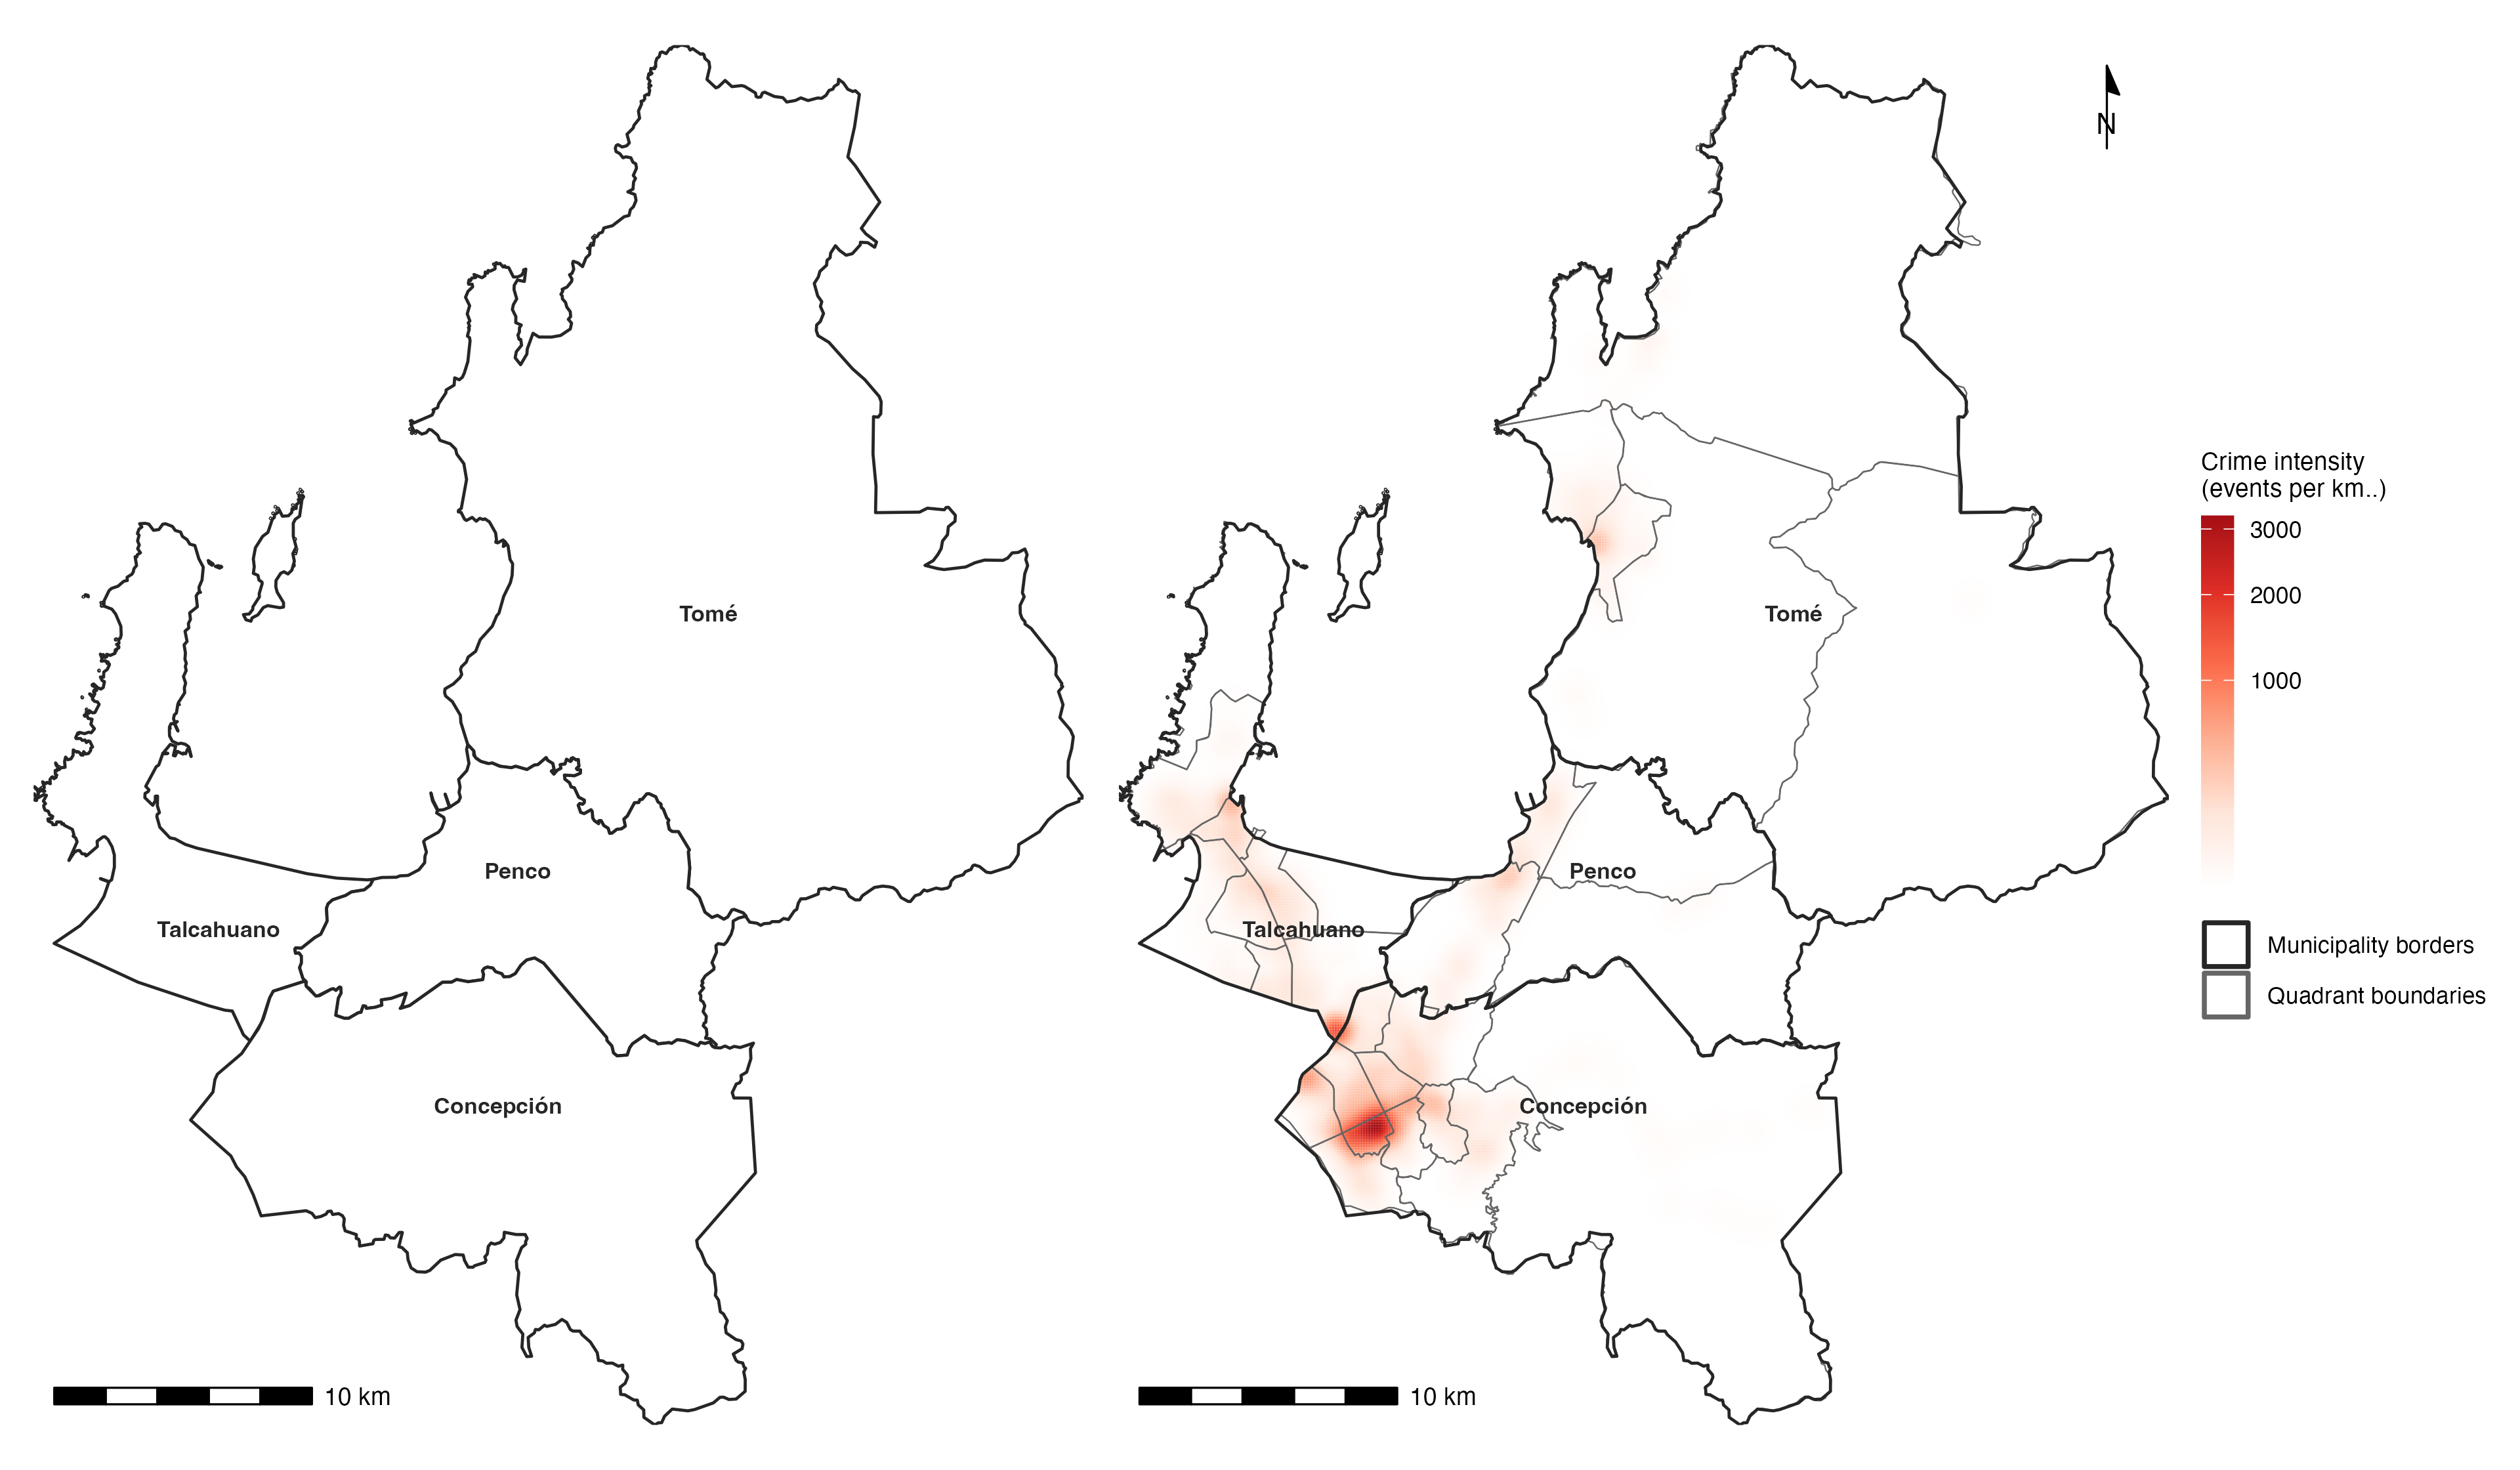
\includegraphics[width=0.62\linewidth]{figures/Graph_PCexample_combined.png}
\end{frame}

% ===================================================================
\section{Data and Empirical Strategy}
% ===================================================================

\begin{frame}{Data}
\begin{columns}[T]
\column{0.5\textwidth}
\textbf{ENUSC survey (INE)}
\begin{itemize}
\item Repeated cross-section, 25,000+ households/year, 101 urban municipalities.
\item Victimization, perceptions, trust, private security investment.
\item Sample: 46 treated (2005--2012) + 1 never-treated municipality.
\item $\sim$27\% of Chile's population.
\end{itemize}
\column{0.5\textwidth}
\textbf{Administrative records}
\begin{itemize}
\item Reported crime (2002--2016) and arrests (2005--2016), \emph{Undersecretary for Crime Prevention}.
\item All Chilean municipalities.
\item Sample: 96 treated (2003--2013) + 196 never-treated.
\item Over half of Chile's population.
\end{itemize}
\end{columns}
\end{frame}

\begin{frame}{Empirical Strategy}
\begin{equation*}
Y_{imt} = \beta_0 + \beta_1\, \text{PC}_{mt} + \mu_m + \mu_t + \varepsilon_{imt}
\end{equation*}
\begin{itemize}
\item Staggered adoption $\Rightarrow$ canonical two-way fixed effects can generate \textbf{negative weights} (Goodman-Bacon).
\item We use \textbf{Callaway and Sant'Anna (2021)}'s estimator for staggered DiD.
\item Robust to alternative staggered-DiD estimators (de Chaisemartin--D'Haultf\oe uille, Gardner, Wooldridge); canonical TWFE attenuates, as expected.
\item Standard errors clustered at the municipality level, wild bootstrap (few, large clusters).
\end{itemize}
\end{frame}

\begin{frame}{Identification}
\begin{itemize}
\item \textbf{Key assumption:} parallel trends absent \PC.
\item Pre-treatment coefficients are small and jointly indistinguishable from zero for all four main outcomes.
\begin{itemize}
\item $p$-values (avg.\ pre-trend $=0$): victimization 0.833; reported crime 0.204; crime perception 0.178; security measures 0.066.
\end{itemize}
\item \textbf{Two main threats:}
\begin{enumerate}
\item Spatial spillovers (Section \ref{spillovers-section}) $\rightarrow$ tested directly, no evidence found.
\item Resource increases confounded with deployment (Section \ref{mechanisms-section}) $\rightarrow$ addressed via heterogeneity analysis.
\end{enumerate}
\end{itemize}
\end{frame}

% ===================================================================
\section{Main Results}
% ===================================================================

\begin{frame}{Victimization and Reported Crime}
\begin{columns}[T]
\column{0.5\textwidth}
\centering
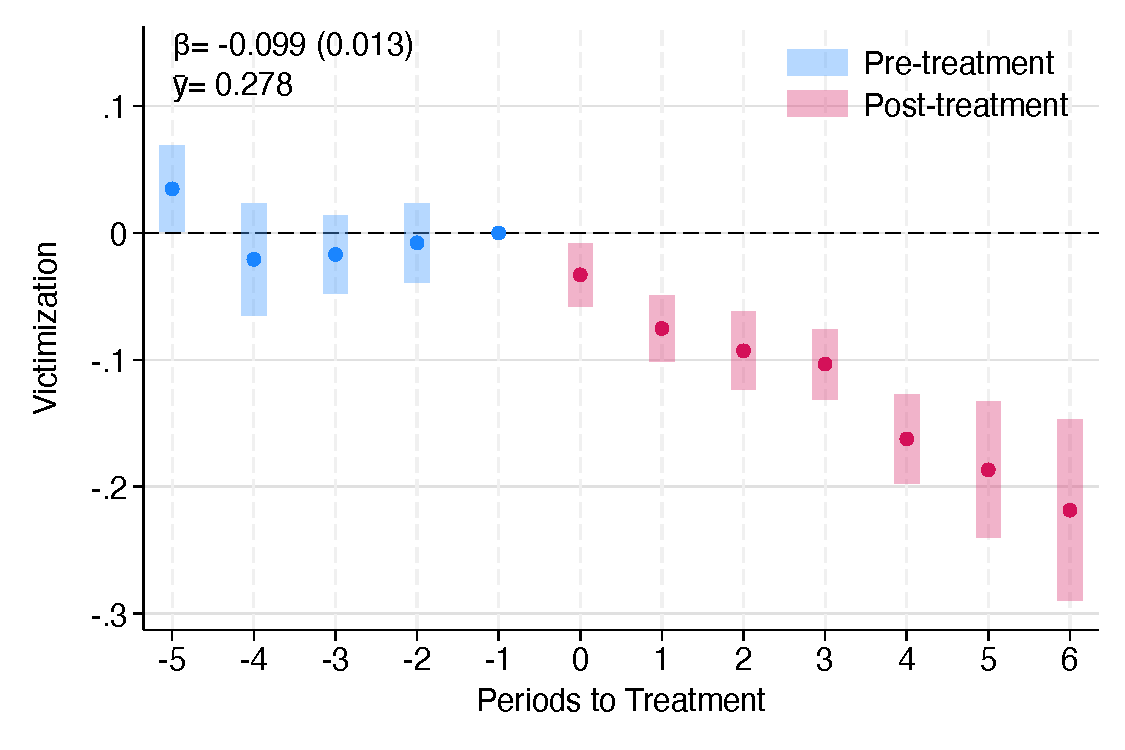
\includegraphics[width=\linewidth]{figures/results_victimization.pdf}\\
\small (a) Victimization (ENUSC)
\column{0.5\textwidth}
\centering
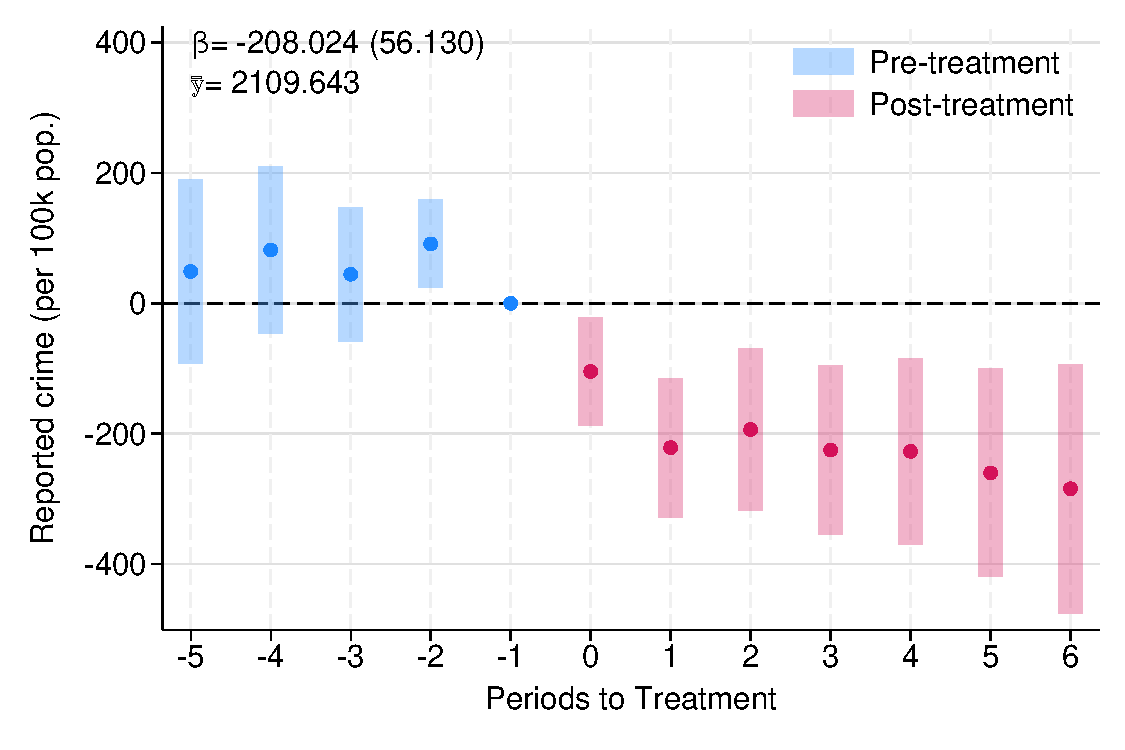
\includegraphics[width=\linewidth]{figures/totalreportedcrime_allcomunas.pdf}\\
\small (b) Reported crime (admin.)
\end{columns}
\begin{itemize}
\item Victimization: $-$10 pp (36\%). Reported crime: $-$208 per 100k (10\%).
\end{itemize}
\end{frame}

\begin{frame}{Crime Perception and Private Security Investment}
\begin{columns}[T]
\column{0.5\textwidth}
\centering
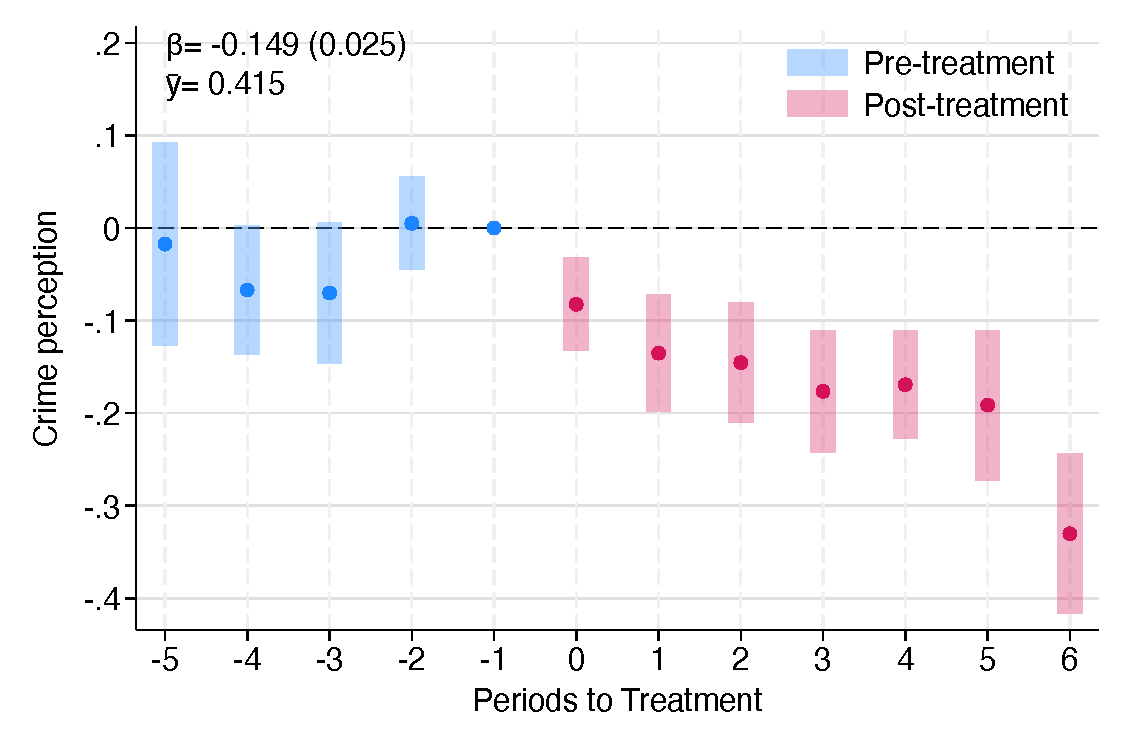
\includegraphics[width=\linewidth]{figures/results_perception.pdf}\\
\small (c) Perceived increase in crime
\column{0.5\textwidth}
\centering
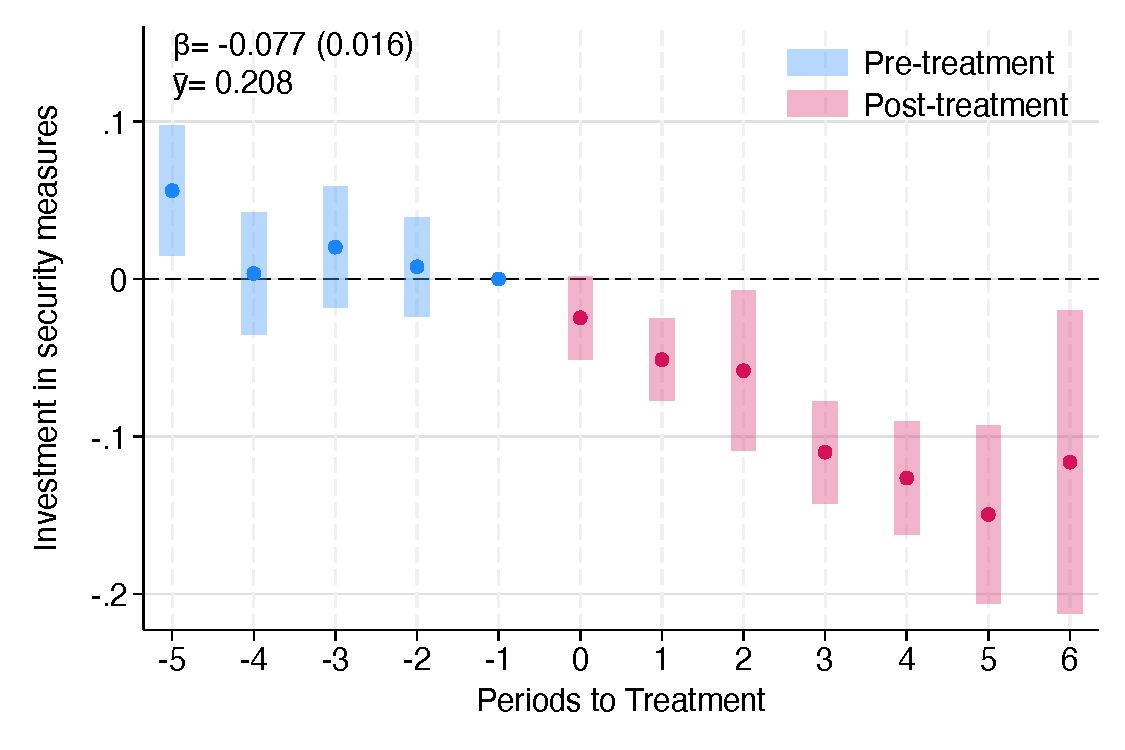
\includegraphics[width=\linewidth]{figures/results_hhprotectionmeasures.pdf}\\
\small (d) Household security measures
\end{columns}
\begin{itemize}
\item Crime perception: $-$15 pp (36\%). Security investment: $-$8 pp (37\%).
\item \textbf{Crime and perceived risk moved together} --- not always the case in the literature.
\end{itemize}
\end{frame}

% ===================================================================
\section{Spillovers}
\label{spillovers-section}
% ===================================================================

\begin{frame}{Are These Effects Really Spillover-Free?}
\begin{itemize}
\item Displacement to neighboring municipalities would bias our estimates \textbf{upward}.
\item \emph{A priori}, spillovers are less likely here:
\begin{itemize}
\item \PC\ reorganizes the \emph{entire} municipal territory, not just crime hot spots.
\item Municipalities are large (avg.\ 101,000 inhabitants, 2,000 km$^2$).
\item Officers are tied to \emph{comisar\'ias} for fixed periods $\Rightarrow$ limited rapid reallocation.
\end{itemize}
\item We test this directly with \textbf{three} complementary exercises.
\end{itemize}
\end{frame}

\begin{frame}{No Evidence of Spillovers to Untreated Neighbors}
\begin{columns}[T]
\column{0.5\textwidth}
\centering
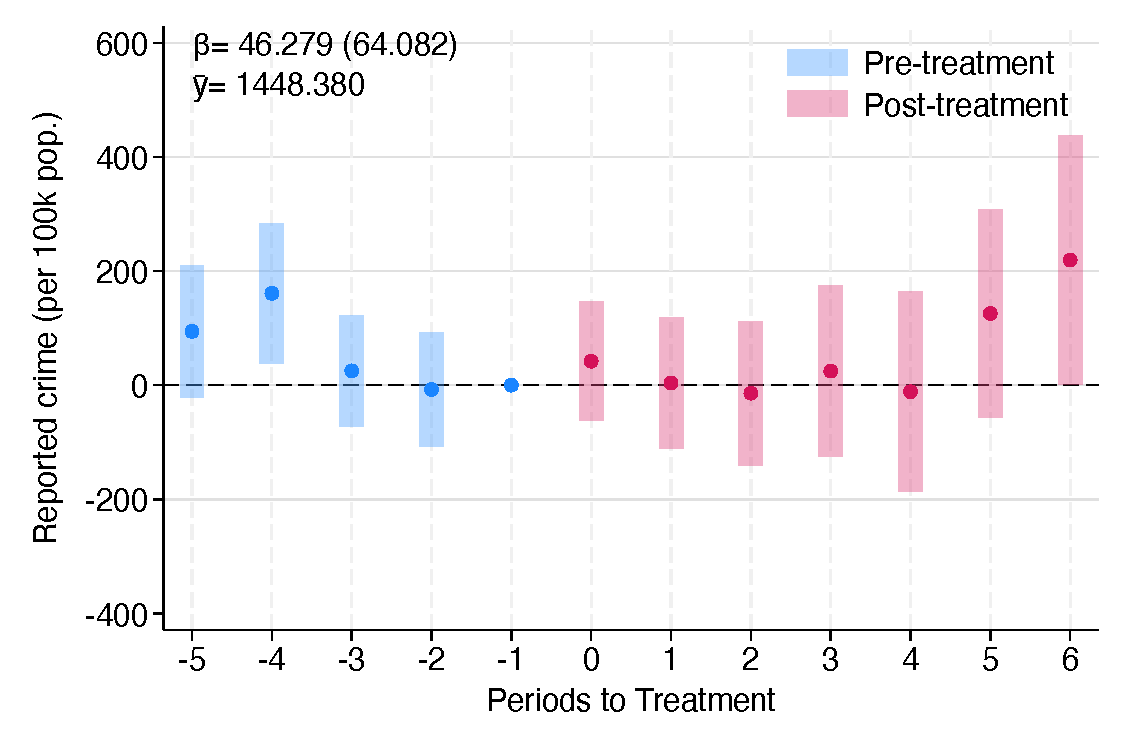
\includegraphics[width=\linewidth]{figures/totalreportedcrime_allcomunas_neighbors.pdf}\\
\small Reported crime: neighbors of adopters
\column{0.5\textwidth}
\centering
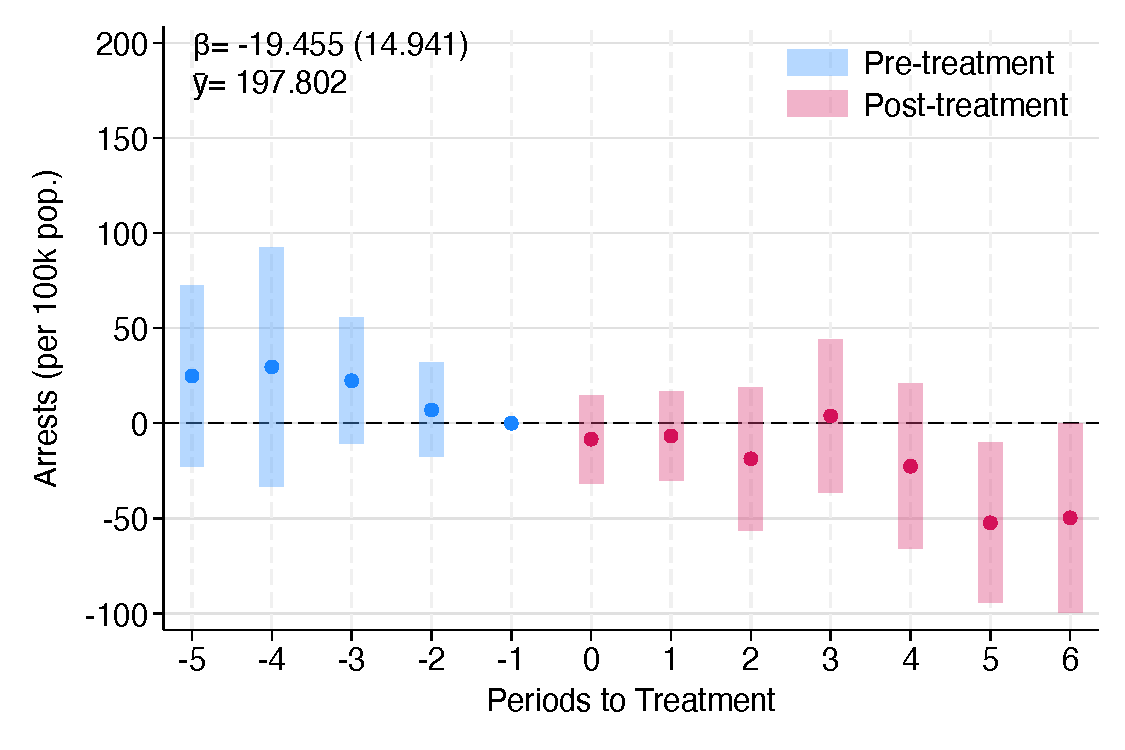
\includegraphics[width=\linewidth]{figures/totalarrestscrime_allcomunas_neighbors.pdf}\\
\small Arrests: neighbors of adopters
\end{columns}
\begin{itemize}
\item Also: continuous exposure (share/number of treated neighbors) and a placebo/permutation exercise --- all null.
\end{itemize}
\end{frame}

% ===================================================================
\section{Heterogeneity}
% ===================================================================

\begin{frame}{Effects Are Broadly Similar Across Municipalities}
\begin{columns}[T]
\column{0.5\textwidth}
\centering
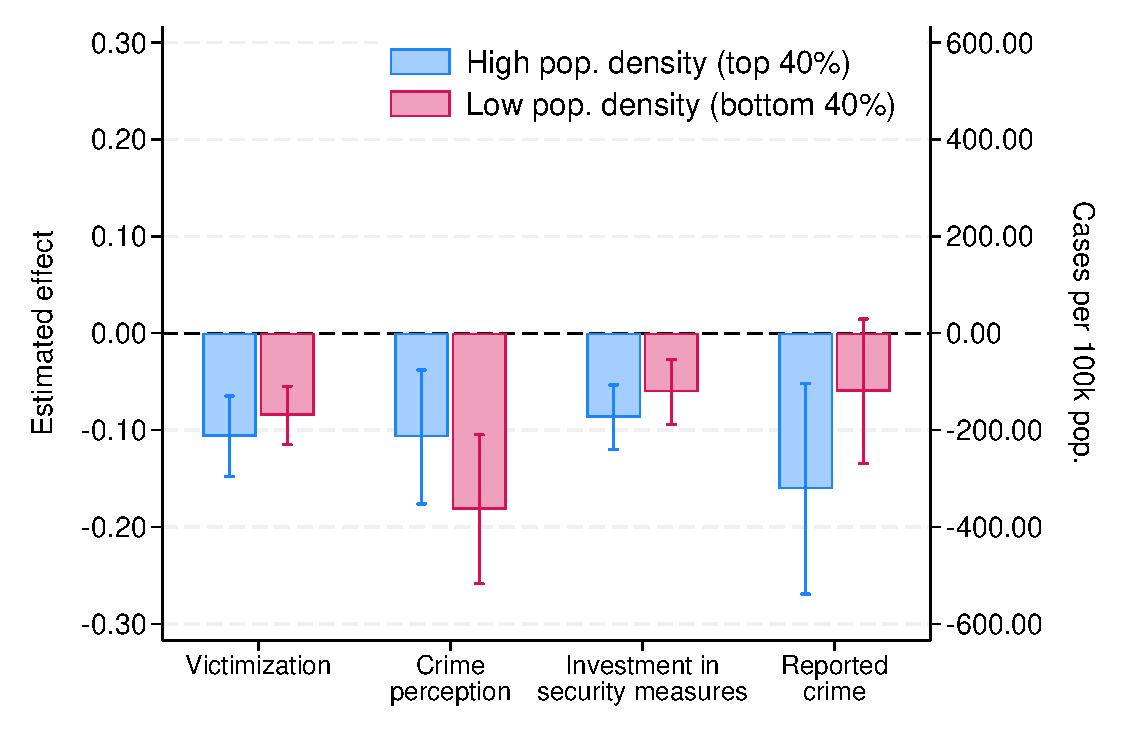
\includegraphics[width=\linewidth]{figures/results_het_density.pdf}\\
\small (a) By population density
\column{0.5\textwidth}
\centering
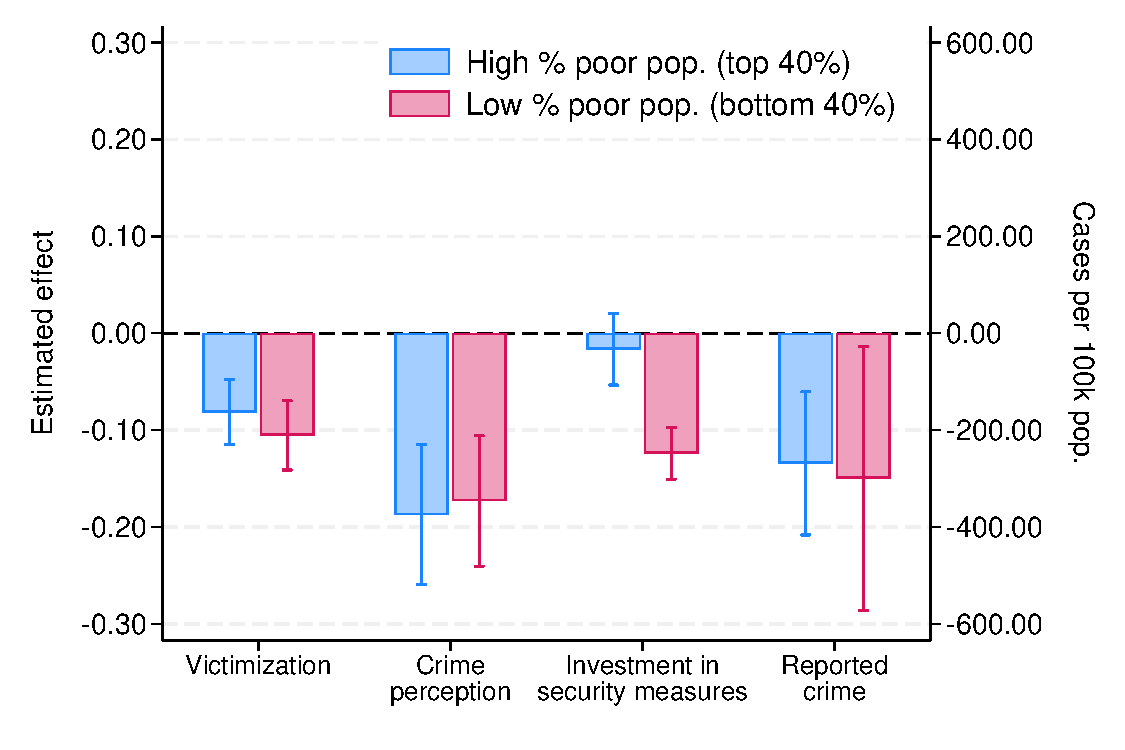
\includegraphics[width=\linewidth]{figures/results_het_poorpop.pdf}\\
\small (b) By poverty rate
\end{columns}
\begin{itemize}
\item Also similar by household socioeconomic status.
\item \textbf{External validity:} gains are not confined to a particular type of municipality or household.
\end{itemize}
\end{frame}

% ===================================================================
\section{What Is Driving the Effects?}
\label{mechanisms-section}
% ===================================================================

\begin{frame}{Confound: \PC\ Also Came with More Resources}
\begin{columns}[T]
\column{0.5\textwidth}
\centering
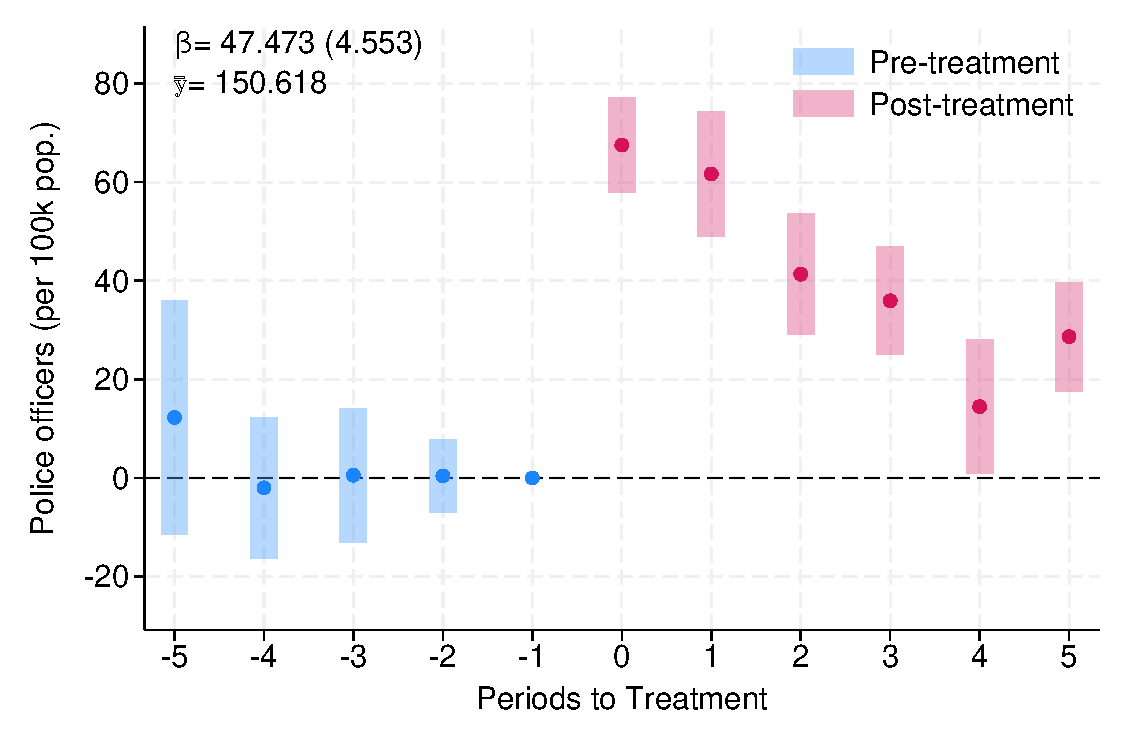
\includegraphics[width=\linewidth]{figures/fig4_officers.pdf}\\
\small (a) Police officers
\column{0.5\textwidth}
\centering
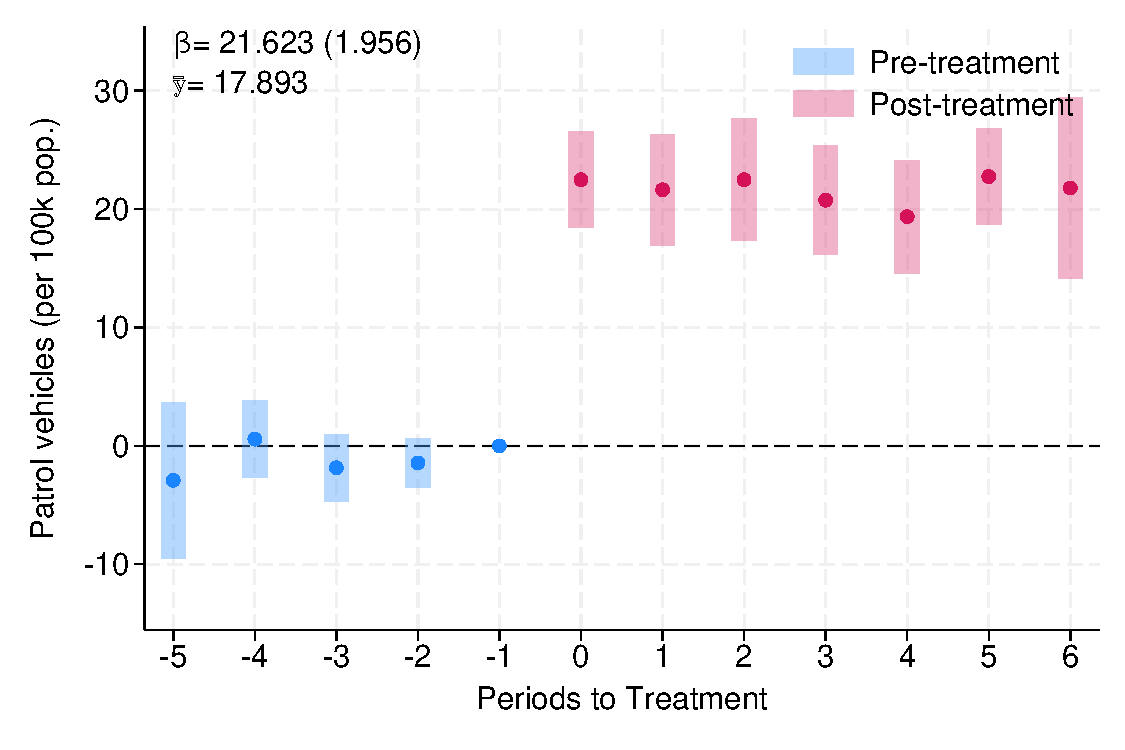
\includegraphics[width=\linewidth]{figures/fig4_patrols.pdf}\\
\small (b) Patrol vehicles
\end{columns}
\begin{itemize}
\item Top-40\% resource-increase municipalities: officers $+$22\%, vehicles $+$80\%, relative to control-like municipalities.
\item \textbf{Question:} are our effects just a resources story?
\end{itemize}
\end{frame}

\begin{frame}{Effects Hold Even Without Differential Resource Increases}
\begin{columns}[T]
\column{0.5\textwidth}
\centering
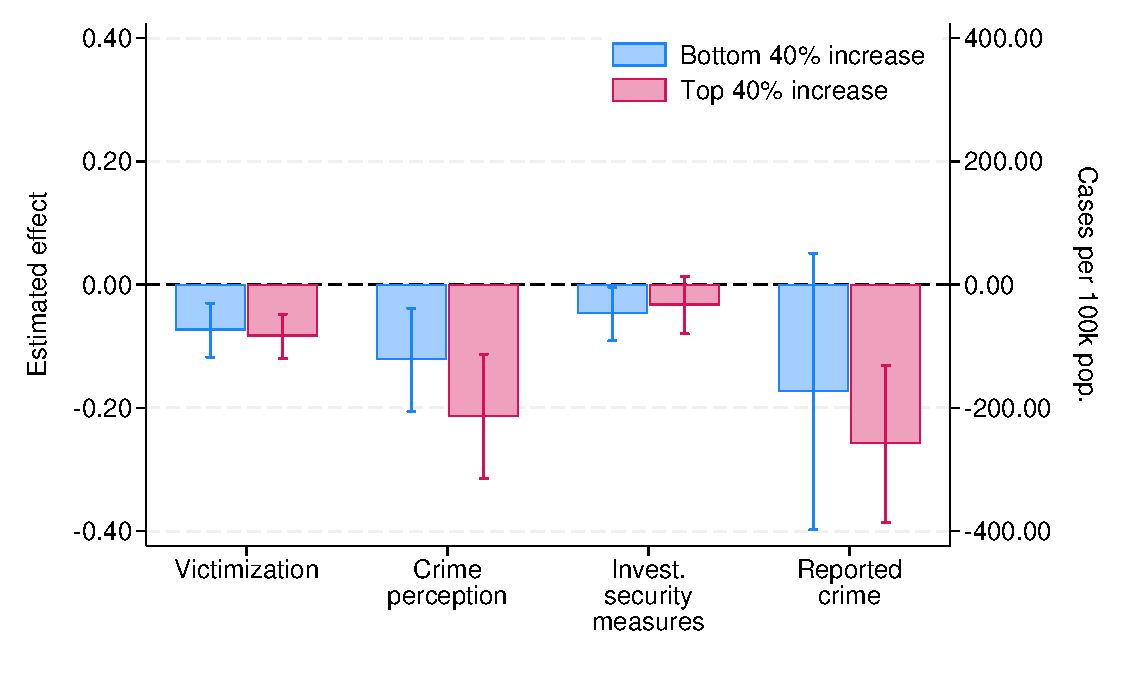
\includegraphics[width=\linewidth]{figures/heterogeneity_off.pdf}\\
\small (e) By intensity of $\Delta$ officers
\column{0.5\textwidth}
\centering
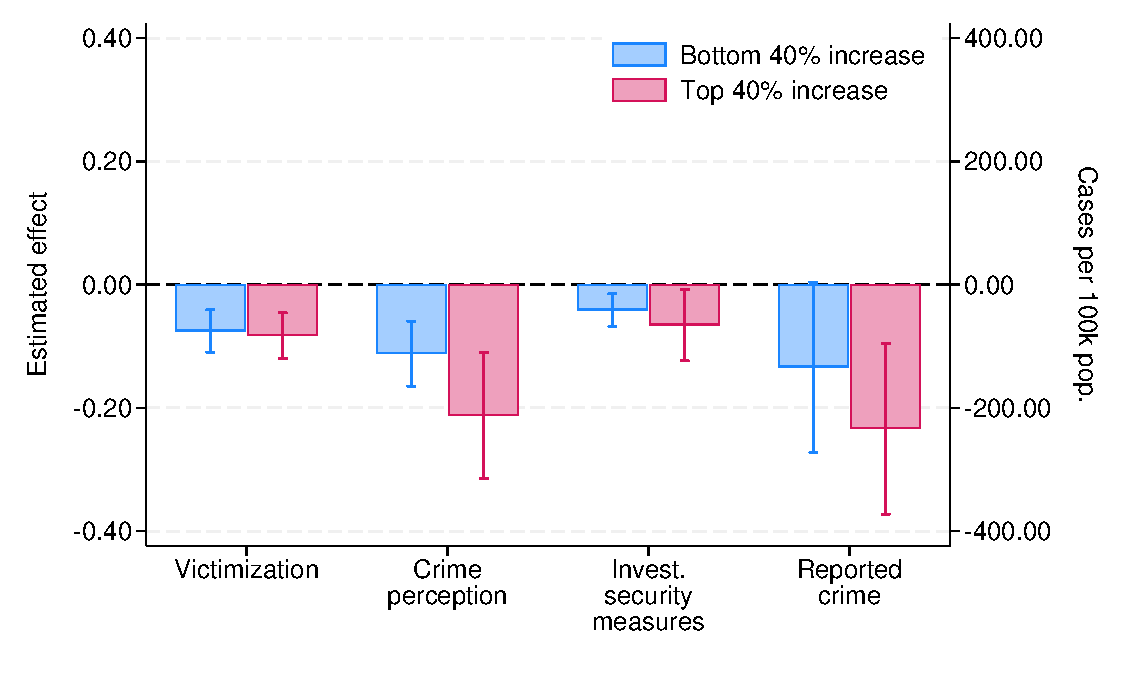
\includegraphics[width=\linewidth]{figures/heterogeneity_pv.pdf}\\
\small (f) By intensity of $\Delta$ patrol vehicles
\end{columns}
\begin{itemize}
\item Bottom-40\% resource-increase municipalities (blue) --- resource growth similar to control group --- still show sizeable effects.
\item Complementary evidence: \emph{Seguridad Ciudadana} (resources w/o deployment change) shows no effect; resource variation \emph{within} already-treated municipalities is unrelated to outcomes.
\end{itemize}
\end{frame}

\begin{frame}{Police Presence and Perceived Performance}
\begin{columns}[T]
\column{0.5\textwidth}
\centering
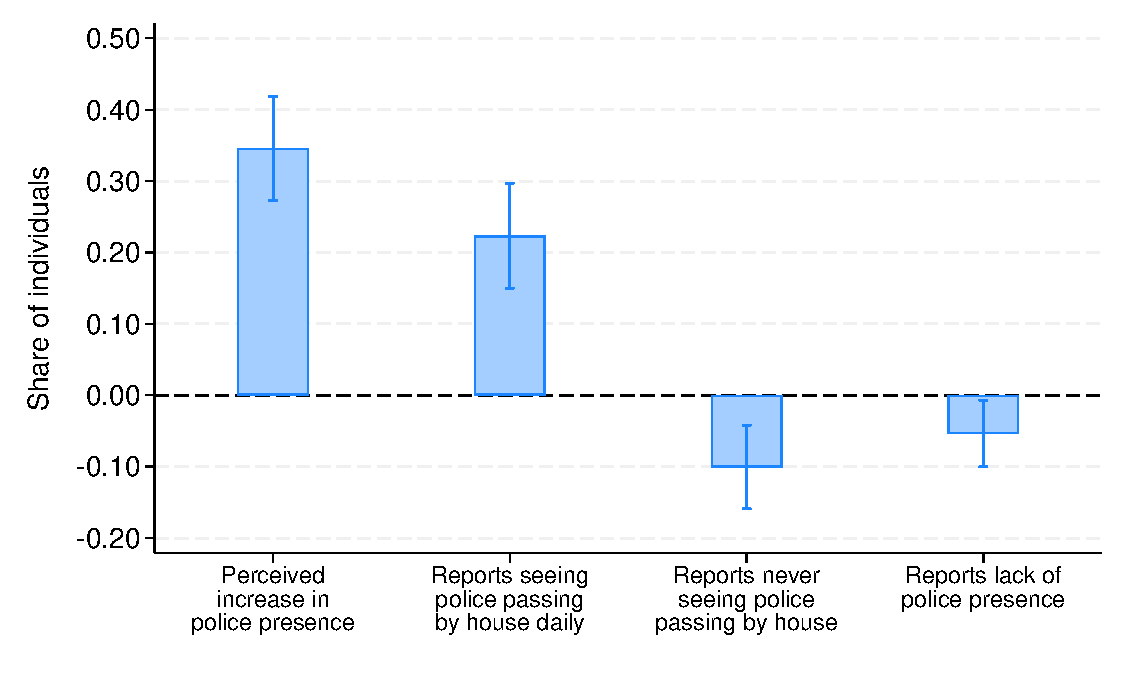
\includegraphics[width=\linewidth]{figures/results_policepresence.pdf}\\
\small (a) Perceived police presence
\column{0.5\textwidth}
\centering
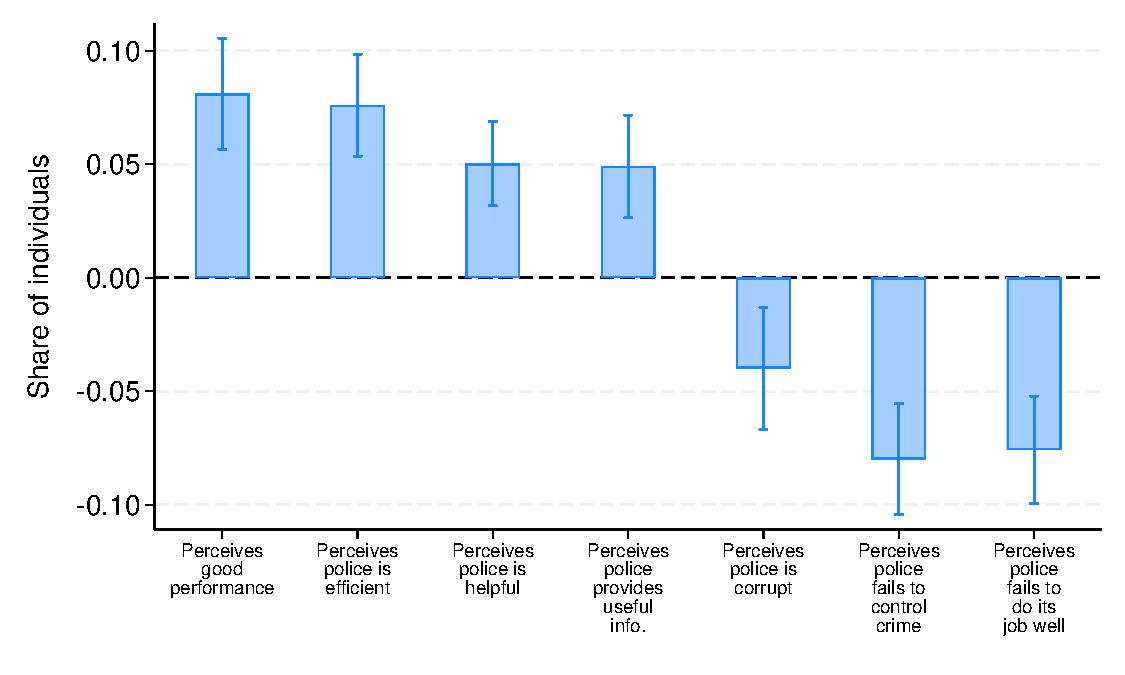
\includegraphics[width=\linewidth]{figures/combined_PCttest_2.pdf}\\
\small (b) Perceived police performance
\end{columns}
\begin{itemize}
\item Perceived police presence: $+$35 pp (156\%). Police rated as good/efficient/helpful/informed $\uparrow$; corrupt/ineffective $\downarrow$.
\end{itemize}
\end{frame}

\begin{frame}{Arrests and Trust: Effectiveness, Not Just Presence}
\begin{columns}[T]
\column{0.5\textwidth}
\centering
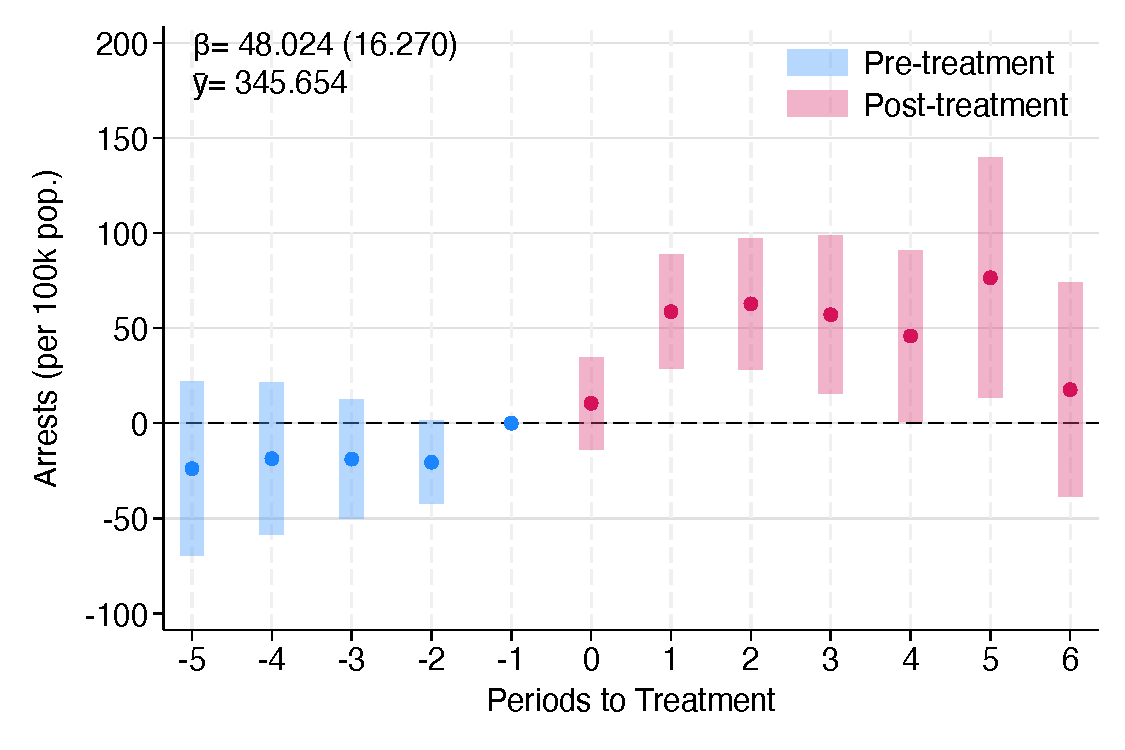
\includegraphics[width=\linewidth]{figures/totalarrestscrime_allcomunas.pdf}\\
\small (c) Arrests (per 100k)
\column{0.5\textwidth}
\centering
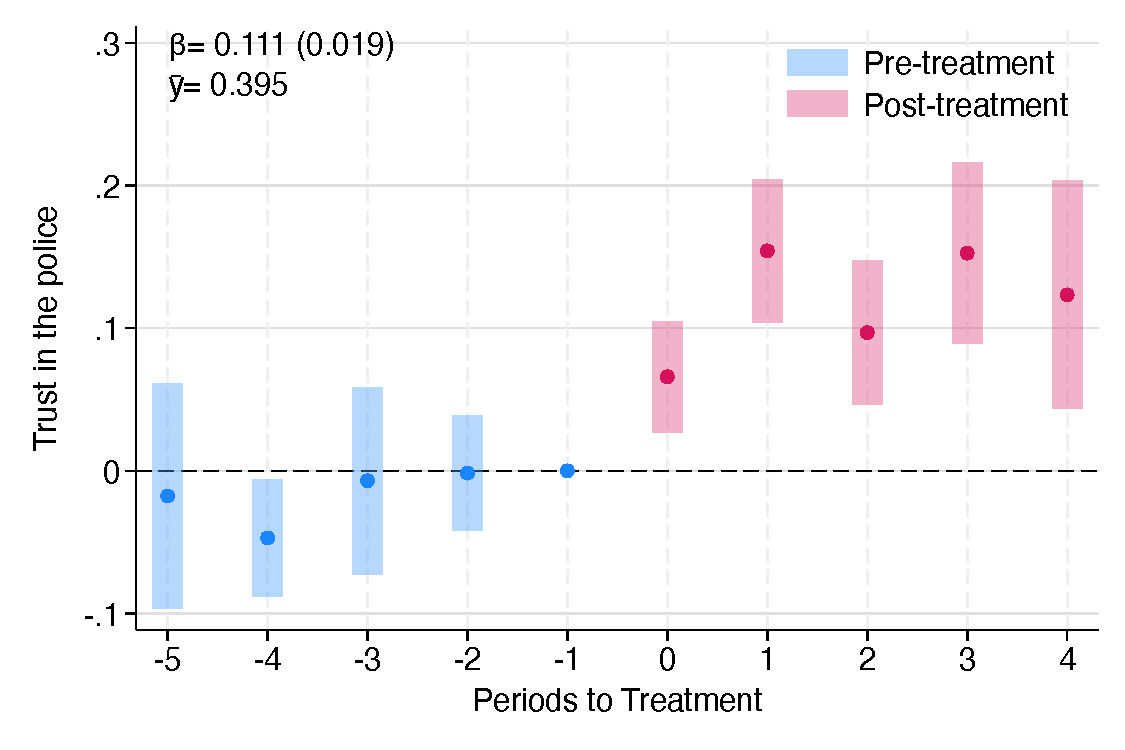
\includegraphics[width=\linewidth]{figures/results_trustcarabineros.pdf}\\
\small (e) Trust in the police
\end{columns}
\begin{itemize}
\item Arrests $+$14\%; arrest/reported-crime ratio $+$1.7 pp (10\%) --- \textbf{while crime is falling}.
\item Consistent with officers building \textbf{local knowledge} under stable territorial assignment, not merely patrolling more.
\end{itemize}
\end{frame}

\begin{frame}{Taking Stock}
\begin{itemize}
\item Resources were likely important for \textbf{implementation}, and may explain part of the effect in some places.
\item But resource increases \textbf{alone} cannot explain our findings:
\begin{itemize}
\item Effects hold where resource growth resembled the control group.
\item A pure-resources reform (\emph{Seguridad Ciudadana}) shows no effect.
\item Arrests rise \emph{while crime falls} --- hard to reconcile with more patrolling alone.
\end{itemize}
\item The evidence points to \textbf{permanent territorial assignment and local knowledge} as key drivers.
\end{itemize}
\end{frame}

% ===================================================================
\section{Conclusion}
% ===================================================================

\begin{frame}{Conclusion}
\begin{itemize}
\item \textbf{Beat policing} --- permanent, small-scale territorial assignment --- generates large gains in public safety \textbf{and} security perceptions.
\item Crime and perceived risk fell \textbf{together}, avoiding the over-investment in private security that misaligned risk perceptions can cause.
\item Trust in the police rose --- notoriously hard to achieve in middle-income settings.
\item The gains are \textbf{not} simply bought with more resources: \textbf{how} police are deployed matters.
\end{itemize}
\end{frame}

\begin{frame}{When Should We Expect Beat Policing to Work?}
\begin{itemize}
\item \PC\ operated in a specific institutional context:
\begin{enumerate}
\item Low organized-crime presence $\Rightarrow$ officers could stay in an area without intimidation risk.
\item A professionally trained police force $\Rightarrow$ capacity to implement the reform well.
\end{enumerate}
\item Neither feature is unique to Chile --- both are present, or attainable, in many settings.
\item \textbf{Policy takeaway:} reorganizing \emph{deployment} can be a cost-effective complement (or alternative) to simply adding more police resources.
\end{itemize}
\end{frame}

\begin{frame}
\centering
{\Large Thank you!}\\[12pt]
\small Comments and questions welcome. \\[6pt]
jorge.garciah@uam.es
\end{frame}

% ===================================================================
\appendix
\section*{Backup Slides}
% ===================================================================

\begin{frame}{Backup: Randomization-Inference Placebo Test}
\begin{columns}[T]
\column{0.5\textwidth}
\centering
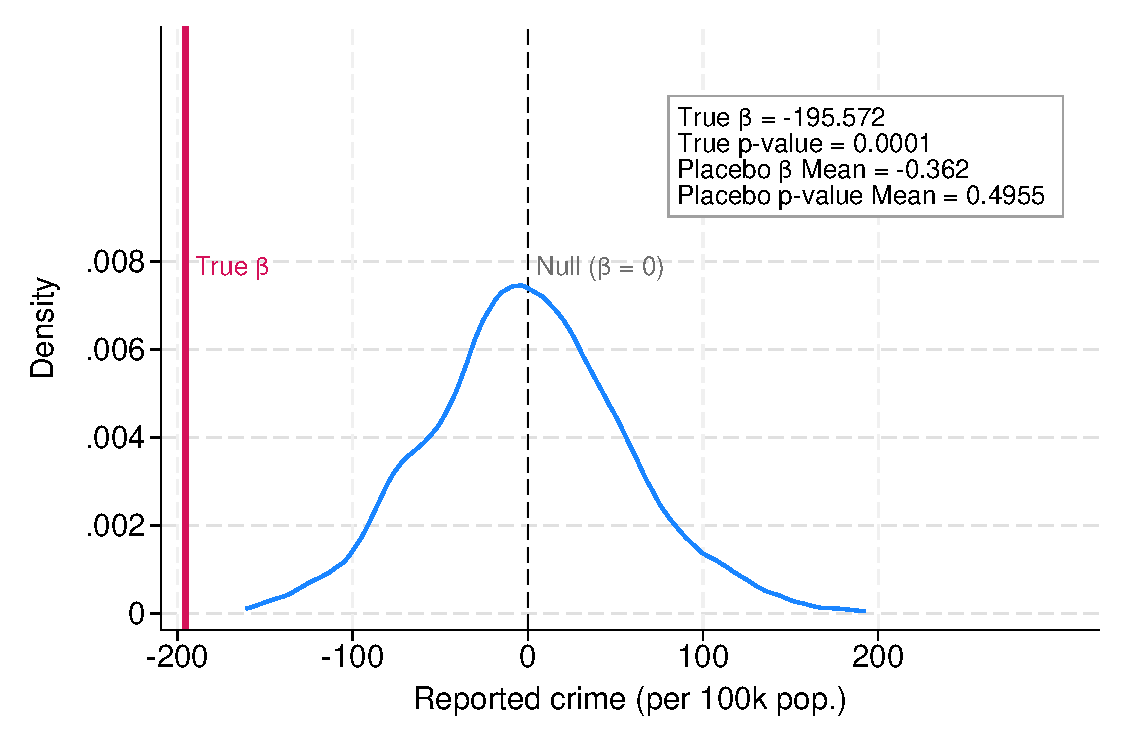
\includegraphics[width=\linewidth]{figures/CHDH_RI_placebo_crime.pdf}\\
\small Reported crime
\column{0.5\textwidth}
\centering
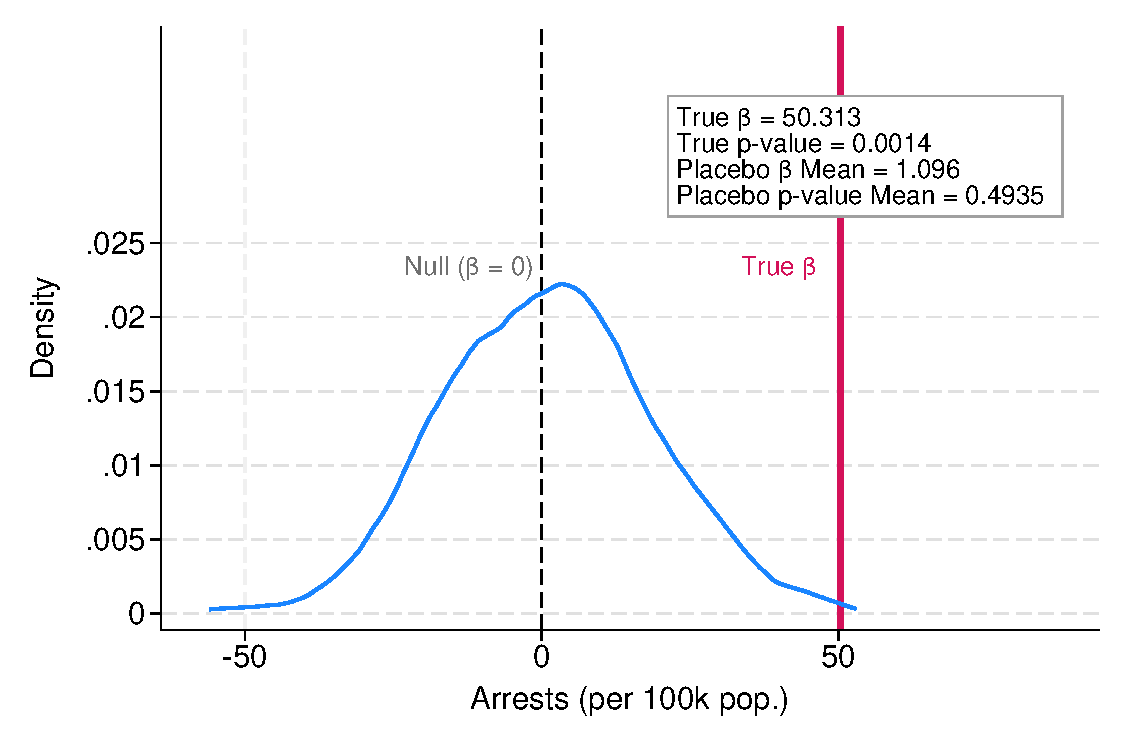
\includegraphics[width=\linewidth]{figures/CHDH_RI_placebo_arrests.pdf}\\
\small Arrests
\end{columns}
\begin{itemize}
\item Placebo distribution from 1,000 random reassignments of adoption dates/never-treated status.
\item True direct effects sit far in the tail of the placebo distribution.
\end{itemize}
\end{frame}

\begin{frame}{Backup: Additional Robustness Checks}
\begin{itemize}
\item Alternative staggered-DiD estimators (de Chaisemartin--D'Haultf\oe uille; Gardner; Wooldridge): similar magnitude and significance.
\item Balanced panel of municipalities: nearly identical estimates.
\item Full (uncapped) event-study window: nearly identical estimates.
\item Bonferroni correction for multiple hypothesis testing: all main results remain significant.
\item Excluding municipalities affected by the 2010 Maule earthquake: nearly identical estimates.
\item Placebo test on non-neighborhood crime (e.g., sexual abuse): no effect, as expected.
\end{itemize}
\end{frame}

\begin{frame}{Backup: Key References}
\begin{itemize}
\item Callaway, B. and Sant'Anna, P.\ (2021). ``Difference-in-Differences with Multiple Time Periods.'' \emph{Journal of Econometrics}.
\item Goodman-Bacon, A.\ (2021). ``Difference-in-Differences with Variation in Treatment Timing.'' \emph{Journal of Econometrics}.
\item Blattman, C., Green, D., Ortega, D., and Tob\'on, S.\ (2021). ``Place-Based Interventions at Scale.'' \emph{Journal of the European Economic Association}.
\item Mastrobuoni, G.\ (2020). ``Police Disruption and Performance.'' \emph{Journal of Public Economics}.
\end{itemize}
\end{frame}

\end{document}
